This work focuses on optimization techniques for processing and
storing metadata in the persistent storage. The solution of our choice
is a MySQL Cluster database, therefore this section will briefly
explain some basic concepts for the reader.

MySQL Cluster is a standard MySQL server with an in-memory clustered
storage engine called NDB
\cite{Ronstrom:2005:RPM:1083592.1083720}. NDB is a real-time,
ACID-compliant, relational database storage engine with no single
point of failure. NDB was designed for the telecom industry where high
throughput and minimum downtime is a necessity. It provides $99.999\%$
uptime with subsecond failure recovery and failover enabled by its
shared-nothing architecture. While the performance is similar to other
NoSQL solutions, 2.5 Million SQL Ops/Sec for MySQL Cluster 7.4 \cite{ndb_benchmark},
it does not lack the features of a relational
database such as ACID transactions, multiple isolation levels with
row-level locking and of course SQL-based declarative query interface.

\begin{figure}
\centering
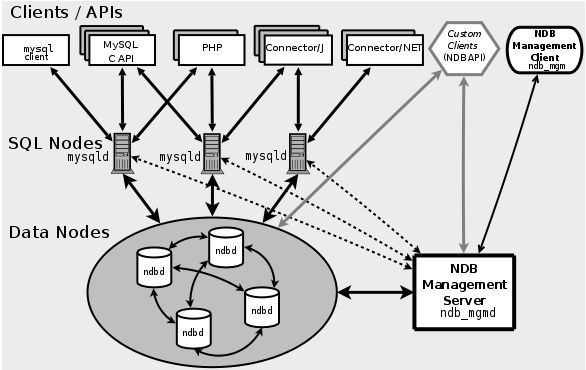
\includegraphics[scale=0.7]{resources/images/Background/ndb_arch.png}
\caption{MySQL Cluster NDB components \cite{ndb_components}}
\label{fig:ndb_ndb_arch}
\end{figure}

A typical MySQL Cluster consists of three entities as illustrated in
Figure \ref{fig:ndb_ndb_arch}. These include:
\begin{description}
\item[Data Nodes] An \texttt{ndb} process that stores the actual data
  -- tables or a
  replica of them. Each Data Node in the cluster should be located in a
  different physical machine.
\item[SQL Nodes] A \texttt{mysqld} server daemon that is used by
  applications to query the schema stored in the cluster.
\item[NDB Management Server] The server which the management client
  connects to in order to perform maintenance operations.
\end{description}

Depending on the the number of Data Nodes and the replication factor,
NDB forms \emph{node groups} such that \textbf{number of node groups}
$=$ \texttt{number of Data Nodes} $/$ \texttt{replication factor}. For example, a
cluster with 8 data nodes and replication factor of 2, will form 4
node groups. Tables in NDB are partitioned by a user-defined key into
these node groups and then replicated in the same group. This
architecture results on data always available with at least one data
node alive in each group. If all data nodes in any group crash, then
the cluster will remain with a corrupted view of the database.
